\documentclass[9pt]{IEEEtran}

\usepackage[english]{babel}
\usepackage{graphicx}
\usepackage{epstopdf}
\usepackage{fancyhdr}
\usepackage{amsmath}
\usepackage{amsthm}
\usepackage{amssymb}
\usepackage{url}
\usepackage{array}
\usepackage{textcomp}
\usepackage{listings}
\usepackage{hyperref}
\usepackage{xcolor}
\usepackage{colortbl}
\usepackage{float}
\usepackage{gensymb}
\usepackage{longtable}
\usepackage{supertabular}
\usepackage{multicol}

\usepackage[utf8x]{inputenc}

\usepackage[T1]{fontenc}
\usepackage{lmodern}{}
\input{glyphtounicode}
\pdfgentounicode=1

\graphicspath{{./figures/}}
\DeclareGraphicsExtensions{.pdf,.png,.jpg,.eps}

% correct bad hyphenation here
\hyphenation{op-tical net-works semi-conduc-tor trig-gs}

% ============================================================================================

\title{\vspace{0ex}
Optical flow}

\author{Marko Medved\vspace{-4.0ex}}

% ============================================================================================

\begin{document}

\maketitle

\section{Introduction}
In this assignment, the mean shift method was first implemented and then
 used to develop a tracker, which was tested on the VOT14 dataset. The model's
  performance was evaluated using different parameters. The tracker was 
  further improved by introducing additional weights for the histogram, 
  with the weights selected based on the tracked object's background.
\section{Experiments}
\subsection{Mean shift mode seeking on the given example}
The Mean Shift method was tested using several different parameters to assess 
its performance. Firstly, the kernel size, which determines the region over which
 the probabilities for making a step are calculated, was varied. Additionally, 
 different starting positions on the density function were considered to evaluate 
 how the initial location affects the results. Lastly, three convergence criteria
  were tested to determine when the iteration should stop: the first, based on step
  size, stops the iteration when the calculated movement is smaller than one pixel; 
  the second, using Euclidean distance, halts the process when the distance between 
  consecutive positions is less than 2 units; and the third, based on change in
   probability, terminates the iteration when the change in the probability 
   distribution is minimal, indicating convergence.

  In Figure~\ref{fig:mode_seeking}, we observe how different combinations of
   these parameters affect convergence. A larger kernel size leads to faster
    convergence, as the calculated steps are generally larger. However, when the 
    kernel size is too small, the algorithm fails to converge to the local maximum 
    because the calculated steps become smaller than a pixel. On the other hand, 
    using an excessively large kernel can also prevent convergence to the local
     maximum, as illustrated by the example with the largest kernel size.

     The starting position is also crucial, as it directly influences the algorithm's
      behavior. If the starting point is located where there is little to no
       probability in the surrounding area, the algorithm will fail to make any 
       steps. Additionally, for functions with multiple local maxima, the starting
        position determines which maximum the algorithm will converge to. 

        Lastly, among the different types of convergence criteria, the sub-pixel 
        step method is generally the most consistent, although it tends to be the
         slowest. It's also worth noting that the "small change in probability" 
         criterion may not always be the best choice, especially if the probabilities 
         change insignificantly at the start, as it can lead to premature convergence. 

\begin{figure}[h]
    \centering
    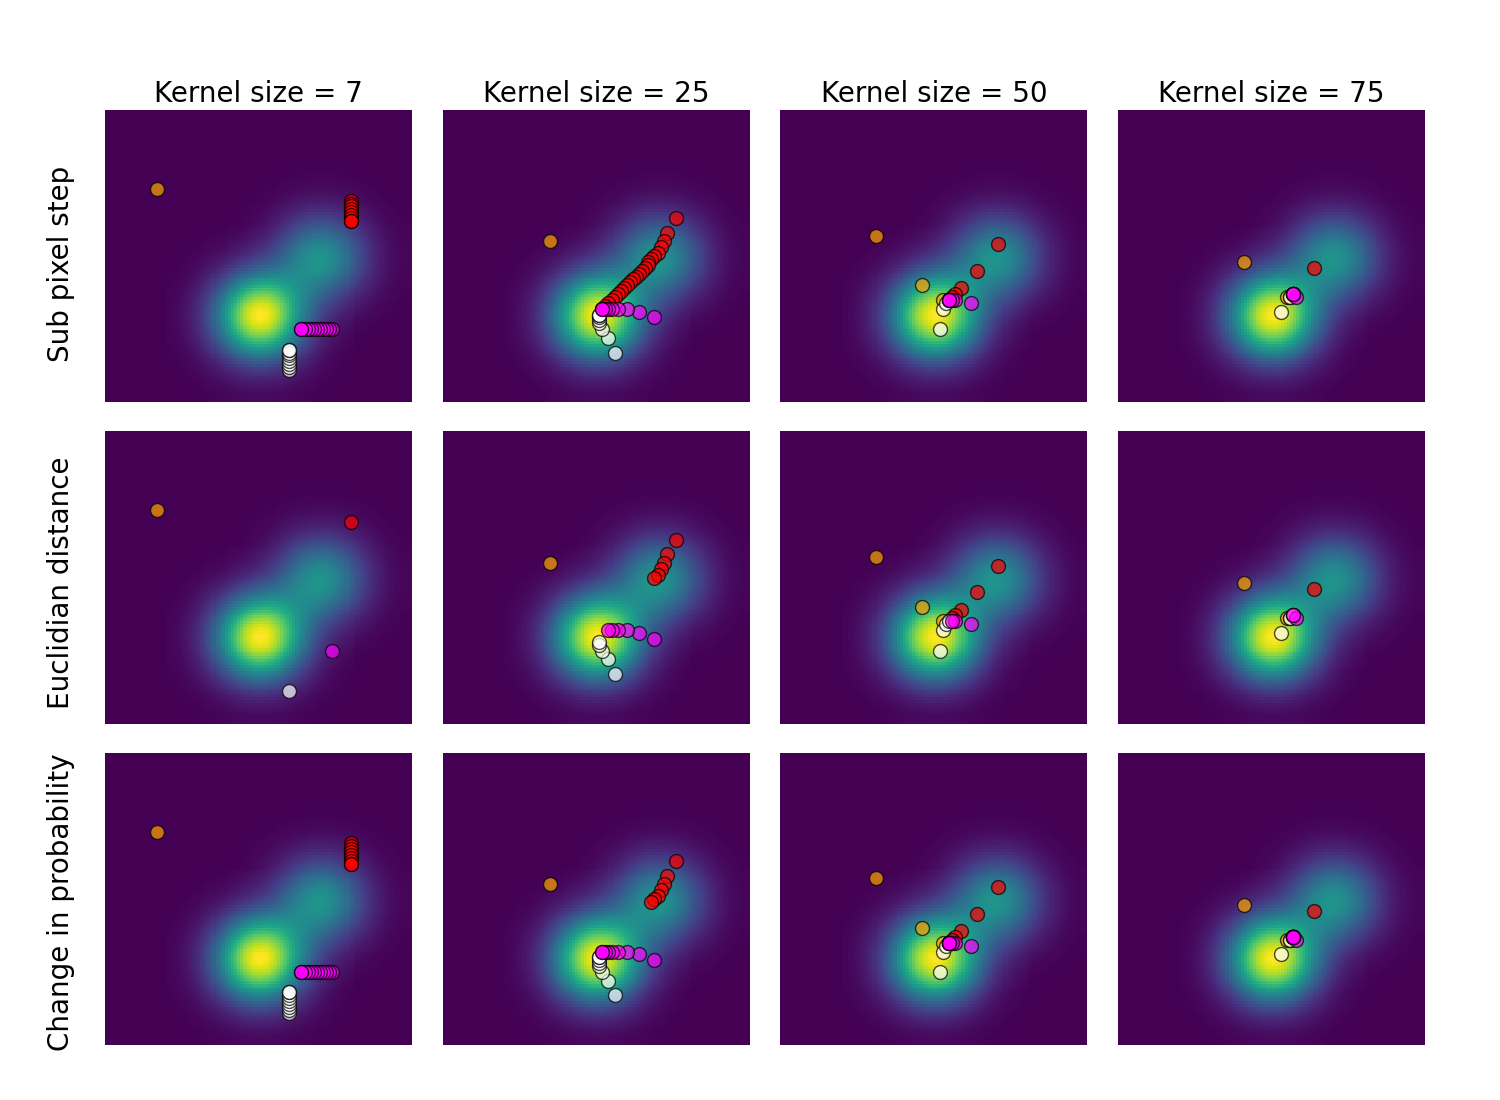
\includegraphics[width=0.99\columnwidth]{figures/mode_seeking.png}
    \caption{Comparison of the mean shift method with different kernel sizes, convergence
    criteria and starting positions}
    \label{fig:mode_seeking}
\end{figure}


\subsection{Mean shift mode seeking on custom examples}
The algorithm was then tested on three custom functions, shown in 
Figure~\ref{fig:mode_seeking2}. In these tests, the sub-pixel convergence criterion
 was used, and the kernel size was set to 25. For each function, four different 
 starting positions were evaluated. The first function is a Gaussian distribution, 
 where the algorithm consistently converges to the global maximum, provided the 
 starting point is not in a region with near-zero probability. The second example 
 is the Laplacian of Gaussian (the Mexican hat function), which has multiple local
  maxima. Here, the convergence outcome strongly depends on the starting position.
   The final example is a small section of the Julian Alps (around 46° North and 
   14° East). Due to the presence of many local maxima, the starting position 
   determines which peak the algorithm will ascend to. 

\begin{figure}[h]
  \centering
  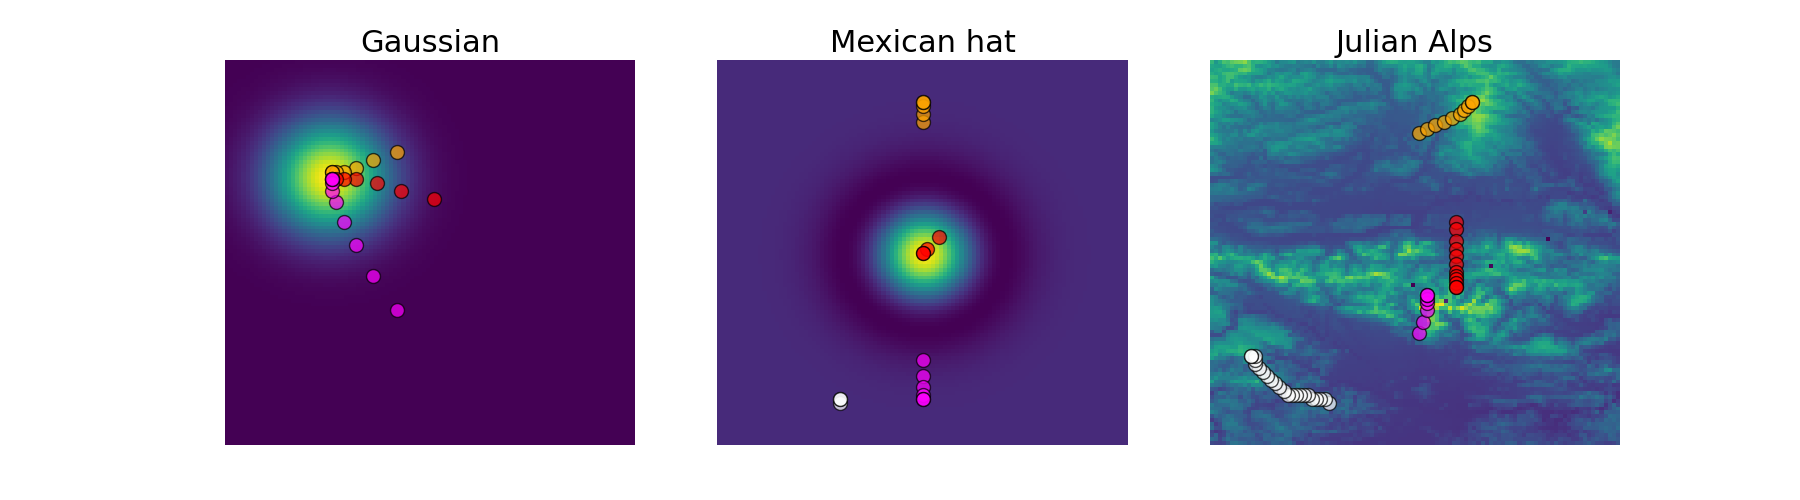
\includegraphics[width=0.99\columnwidth]{figures/mode_seeking2.png}
  \caption{Comparison of the mean shift method on different functions}
  \label{fig:mode_seeking2}
\end{figure}

\subsection{Basic tracker implementation}
The tracker was implemented and tested on the entire VOT 2014 dataset. 
The number of failures and the tracking speed (measured on my personal laptop)
 are summarized in Table~\ref{tab:basic_tracker_results}. Overall, the tracker 
 failed a total of 33 times across the dataset. While the tracker performs reliably
  in most cases, it struggles more with certain sequences, such as hand2, fish1,
   torus, and tunnel. The reasons behind these failures will be explored in detail in the next section. 

\begin{table}[ht]
  \centering
  \caption{Basic Tracker Results}
  \setlength{\tabcolsep}{3pt}
  \begin{tabular}{l|c|c||l|c|c}
  \hline
  \textbf{Sequence} & \textbf{Failures} & \textbf{Speed} & \textbf{Sequence} & \textbf{Failures} & \textbf{Speed} \\ 
  \hline
  ball       & 1 & 1823 FPS & david     & 1 & 1042 FPS \\ 
  basketball & 0 & 510 FPS  & diving    & 0 & 1328 FPS \\ 
  bicycle    & 1 & 1047 FPS & drunk     & 1 & 700 FPS  \\ 
  bolt       & 2 & 1425 FPS & fernando  & 2 & 358 FPS  \\ 
  car        & 0 & 2017 FPS & fish1     & 3 & 1571 FPS \\ 
  fish2      & 1 & 1224 FPS & motocross & 2 & 504 FPS  \\ 
  gymnastics & 0 & 1667 FPS & polarbear & 0 & 2020 FPS \\ 
  hand1      & 2 & 923 FPS  & skating   & 1 & 1098 FPS \\ 
  hand2      & 5 & 2610 FPS & sphere    & 0 & 1285 FPS \\ 
  jogging    & 1 & 1704 FPS & sunshade  & 0 & 928 FPS  \\ 
  surfing    & 0 & 3179 FPS & torus     & 3 & 1170 FPS \\ 
  trellis    & 2 & 1449 FPS & tunnel    & 4 & 2684 FPS \\ 
  woman      & 1 & 2525 FPS &           &   &          \\ 
  \hline
  \end{tabular}
  \label{tab:basic_tracker_results}
  \end{table}
  
  
  \subsection{Failure cases discussion}
  The cases where the tracker experienced the most failures are shown in 
  Figure~\ref{fig:failures}. In the fish1 and hand2 sequences, the failures 
  occurred because the color distributions of the bounding box being tracked
   were very similar to those of the ground truth bounding box, making it difficult
    for the tracker to detect movement. While the failures in the other two 
    sequences, torus and tunnel, are less obvious, they can be interpreted in a similar way, with the added complexity of scale changes in both videos. In the torus sequence, as the object rotated around its axis, the color distribution of the tracked patch changed significantly, leading to tracking failure. In the tunnel sequence, when the motorbike moved further away from the camera, its scale decreased, causing the bounding box to become too large and inaccurate.

  These failure cases suggest two potential improvements for the tracker. 
  First, the issue with scale changes could be mitigated by trying different
   template scales and selecting the one that provides the most similarity.
    Second, the tracker could be improved by addressing the influence of the 
    background, which is a factor that will be discussed in more detail in the
     final section.

  \begin{figure}[h]
    \centering
    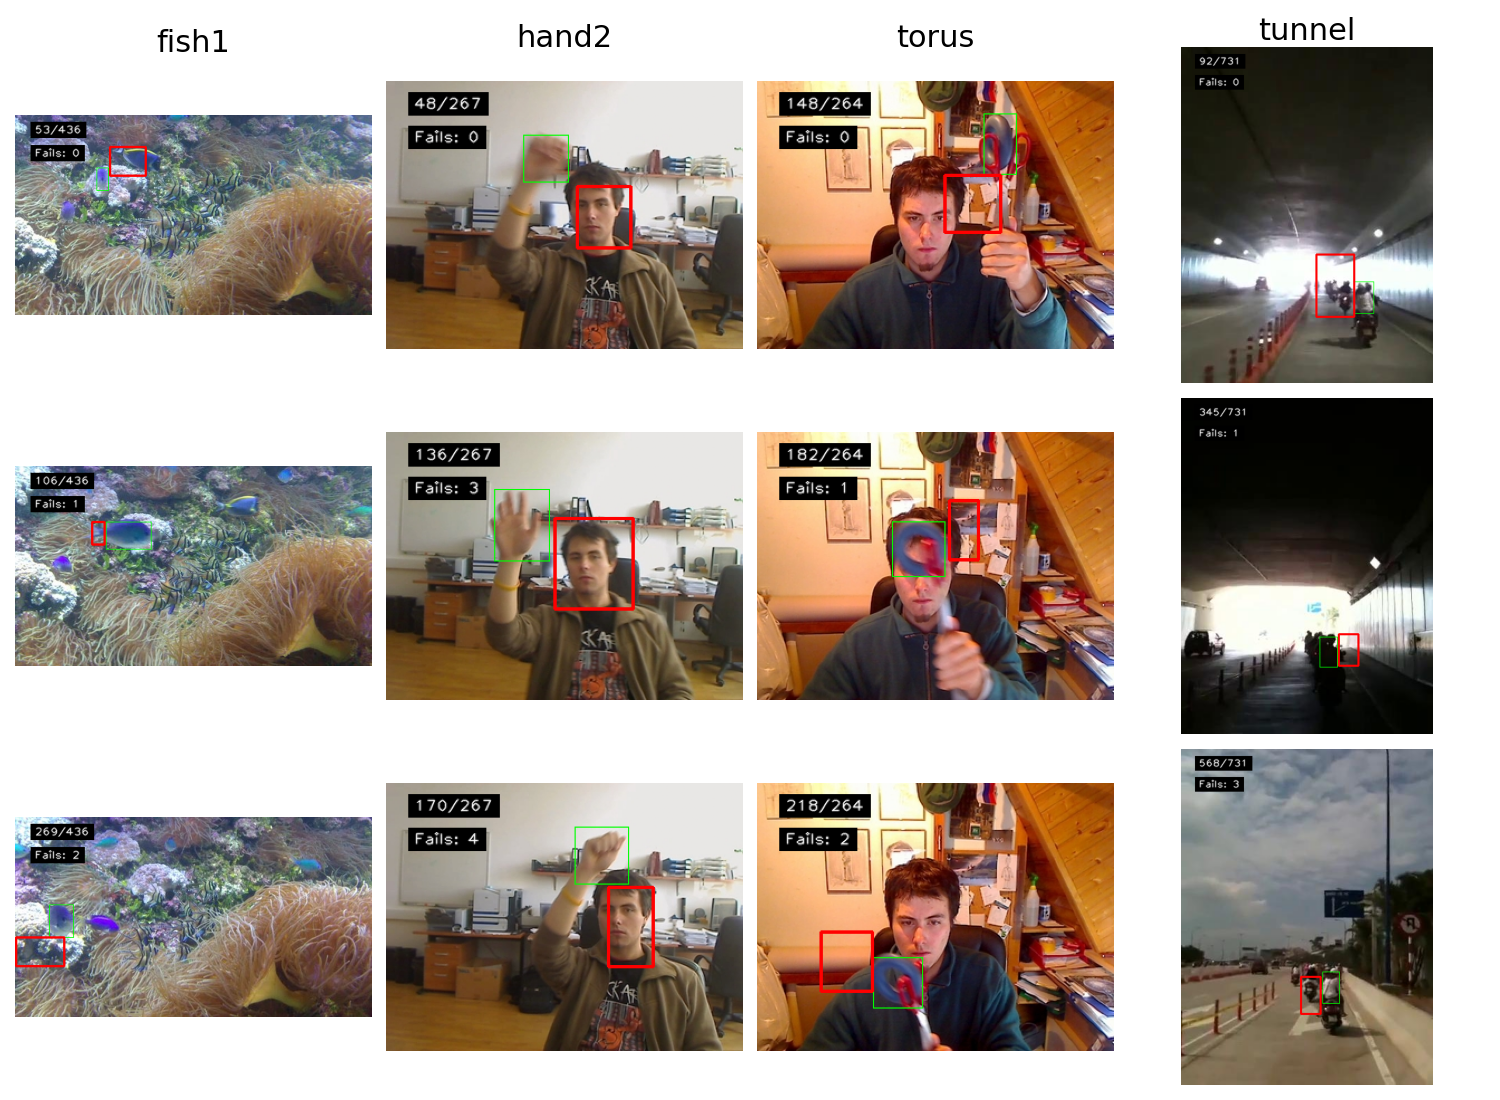
\includegraphics[width=0.99\columnwidth]{figures/failures.png}
    \caption{Mean shift tracker failure cases}
    \label{fig:failures}
  \end{figure}

\subsection{Parameter tuning}
Four key parameters were considered: $\sigma$(kernel size), the number of bins in 
the histograms, the number of iterations per frame, and $\alpha$(the update rate of the template).
 The algorithm was tested on all combinations of 4 different bin counts, 4 different 
 kernel sizes, 3 iteration values, and 4 update rates.

To determine the optimal number of iterations and bins, the results were aggregated 
based on these two parameters, as shown in Figure~\ref{fig:params1}. The data indicates 
that using only one iteration significantly reduces performance, whereas 10 and 20
 iterations produce similar results. The average FPS for 10 and 20 iterations was 1482 
 and 1484, respectively, showing negligible difference in processing speed.

Regarding the number of bins, it is clear that 8 or 16 bins provide the best performance.
 Although 8 bins slightly underperform compared to 16, they offer a noticeable increase
  in average FPS. However, on my personal laptop, the average FPS for 16 bins reached
   2151, making it the preferred choice unless running on a computationally limited
    device.

Based on these findings, the optimal settings are 20 iterations and 16 bins, as 
this combination minimizes failures while maintaining high processing speed. These values 
will be used for further evaluation.

 \begin{figure}[h]
  \centering
  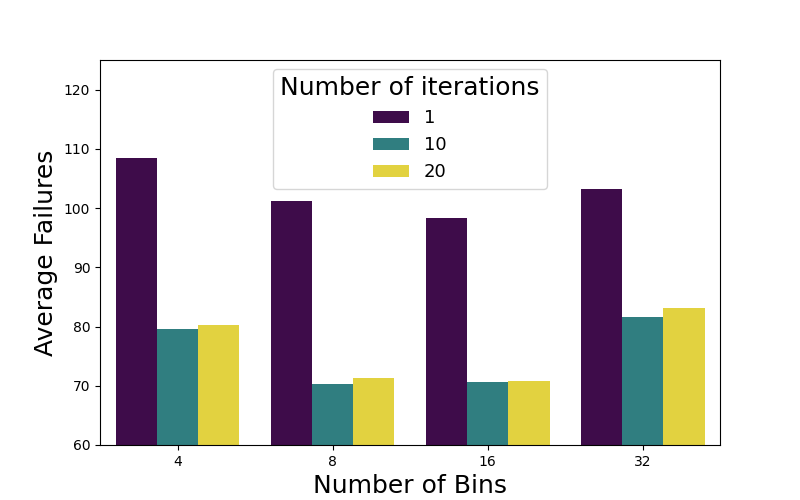
\includegraphics[width=0.99\columnwidth]{figures/nbins_niters.png}
  \caption{Performance of the means shift tracker with different numbers of bins and numbers of
  iterations}
  \label{fig:params1}
\end{figure}

To determine the best values for $\sigma$ and $\alpha$, we refer to Figure~\ref{fig:params2}. 
Since the FPS remains relatively consistent across different values of these parameters, the 
focus is on minimizing the number of failures. The results suggest that the optimal value for
 $\sigma$ is clear. However, the choice of $\alpha$ may be more problem-specific, as the average
  performance is quite similar across the entire dataset. For scenarios where the target is
   expected to change frequently, $\alpha = 0.01$ is likely the better choice, whereas for more
    stable targets, $\alpha = 0$ would be more suitable.

\begin{figure}[h]
  \centering
  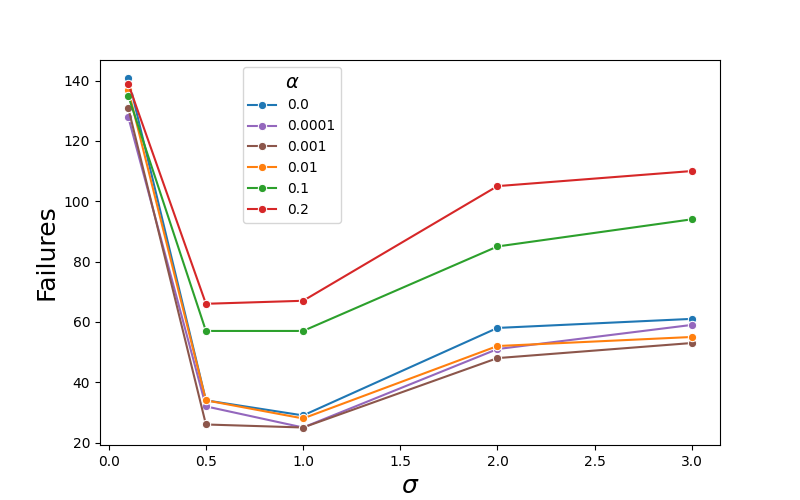
\includegraphics[width=0.99\columnwidth]{figures/sigma_alpha.png}
  \caption{Performance of the means shift tracker with different kernel sizes and update rate
  parameters}
  \label{fig:params2}
\end{figure}

\subsection{Feature selection by accounting for the background in different color spaces}
To address the background influence, the method applied smaller weights to the
 regions in the histogram where the background color predominated. The tracker
  was also evaluated using five different color spaces. Additionally, another
   parameter was introduced: the size of the background area. Since the optimal 
   value for alpha was not definitive in the previous evaluation, two potential 
   alpha values (0 and 0.01) were also considered in this experiment.  


\section{Conclusion}


\bibliographystyle{IEEEtran}
\bibliography{bibliography}

\end{document}
